\section{Simulation Study}\label{sec:eval}

In this section, we present preliminary results of a simulation study on the
effectiveness of removing redundant messages.

\subsection{Experiment Setup}

We conduct experiments on a simulator of the proposed system.  We simulate a
datacenter network of $1,000$ machines.  It consists of $50$ racks, with $20$
machines in each rack.  Bandwidth quotas and receiver replication are not
enabled.  The receiver node has $4$Gbps bandwidth available; all other machines
have a $1$Gbps network connection.  The latency between a pair of machines is
fixed at $1$ms.

We run the simulation using a web caching workload.  Each message is $32$ bytes
long, and contains an integer which represents an object ID being updated.  The
keys are drawn from a Zipf distribution with the skew parameter set to $1.1$.
This distribution is commonly used to model web caching
workloads~\cite{BCFPS99, CSTRS10, HBvRLKL13}.

A simple rule is applied to data compaction: if multiple messages contain the
same object ID, only one of them is necessary to be forwarded.  In such cases,
the message with earliest timeout is forwarded for performance.

\subsection{Bandwidth Saving from Data Compaction}

The first set of experiments examines the bandwidth saving brought by
discarding redundant messages.  We change the total message delay, and
observe the percentage of bandwidth can be saved.  The fanout is fixed to 4.
We show the results from using one tree and multiple trees ($3$ in this case).
All the rack hubs perform data compaction.  The message delay is distributed
evenly across all the tree levels.

Two workloads are used.  In the heavier workload, each node generates $15,000$
messages per second, that is $457.8$MB per second across the whole datacenter.
Each node generates $3,000$ messages in the other workload, that is $91.6$MB
per second in total.

Figure~\ref{fig:savings} shows the results under two workloads using one and
multiple trees.  All the curves go upwards as total message delay increases, as
longer delays allow more messages to be accumulated at each tree node,
increasing the opportunity for detecting redundant messages.  Also, higher
workload results in more bandwidth savings, since within the same delay period,
more messages are accumulated.  Within the same level of workload, the use of
multiple trees negatively affects bandwidth saving.  This is because as
messages being forwarded through multiple paths, there are fewer messages,
therefore saving opportunities, along each path.

\begin{figure}[t]
\begin{center}
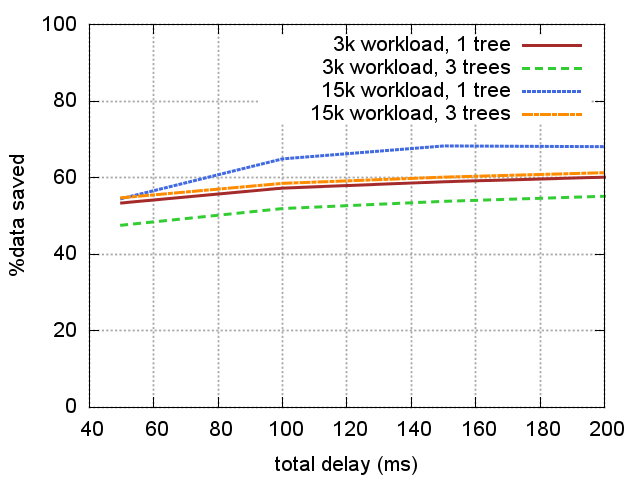
\includegraphics[width=3in]{img/savings.png}
\end{center}
\caption{\label{fig:savings} Effect of changing total message delay on
bandwidth savings.}
\end{figure}

We also evaluate the \emph{effective throughput} of aggregation with data
compaction for the same set of experiments.  The \emph{effective throughput} is
defined as total throughput including messages that are not forwarded due to
data compaction.  Figure~\ref{fig:eff-tp} shows the results. 

The two workload are chosen such that without data compaction, all the messages
generated by the lighter workload could fit into the $1$Gbps bandwith, whereas
the heavier workload well exceeds this bandwidth.  We see that regardless of
whether multiple trees are enabled, the effective throughput of the lighter
workload are almost identical, and they stayed flat with respect to changing
message delays.  This is because virtually all the messages can get through the
system, dispite the actually saving numbers differ, as shown in
Figure~\ref{fig:savings}.  The small difference between the two curves is
caused by queueing overhead.

The two curves of the heavier workload reflectsthe effect of data compaction.
It is not enough to get all the messages through the system using only one
tree.  Therefore, the effective throughput goes up as more delay is injected.
On the other hand, there is enough bandwidth with the help of three trees, and
all the messages can get through the system.

\begin{figure}[t]
\begin{center}
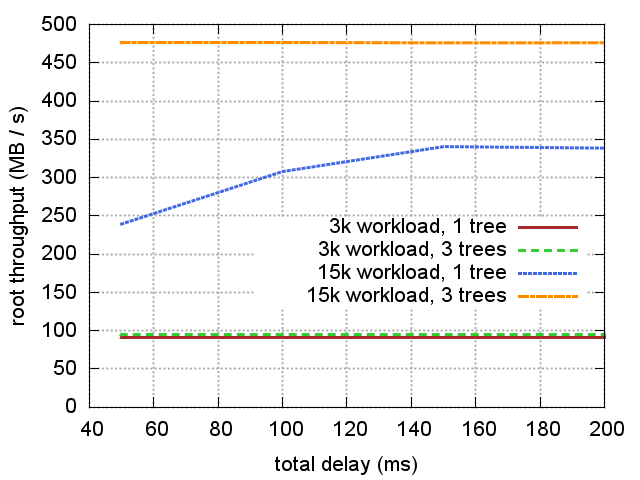
\includegraphics[width=3in]{img/eff-tp.png}
\end{center}
\caption{\label{fig:eff-tp} Effect of changing total message delay on
effective throughput.}
\end{figure}

\subsection{Message Delay Distribution}

This experiment takes a closer look at bandwidth saving from individual nodes,
and the effect of changing the policy of distributing message delay among
nodes.  We used the heavier workload described previously with only one tree.
Data compaction is enabled.  The total message delay is fixed at $100$ms.
Other experiment setup are the same as in the last section.

We include three policies of message delays.  Case $1$ divides the $100$ms
delay uniformly across all the levels in the tree; case $2$ and $3$ distributes
the delay proportionally across tree levels.  In case $2$, the closer a node to
root, the longer delay it gets; case $3$ is the opposite.

\begin{figure}[t]
\begin{center}
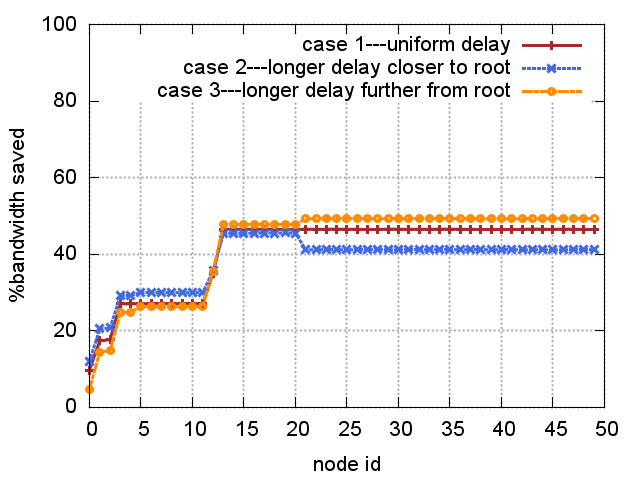
\includegraphics[width=3in]{img/node_saving.png}
\end{center}
\caption{\label{fig:node-saving} Outbound bandwidth of each node with data compaction
enabled.  Nodes are sorted in decreasing bandwidth utilization.}
\end{figure}

Figure~\ref{fig:node-saving} shows the result of bandwidth saving at each
individual node.  Nodes are sorted by the level-order traversal of the tree.
At each particular node, longer delay results in more saving of bandwidth.  In
all cases, the first three levels of the nodes show much less saving
percentages than the leaves.

\begin{table}[h]
\begin{center}
\begin{tabular}{|c|c|c|c|}
\hline
 & Case 1 & Case 2 & Case 3 \\ \hline
Savings & 64.89\% & 67.32\% & 60.97\% \\ \hline
\end{tabular}
\end{center}
\caption{\label{tab:saving} Aggregated bandwidth saving with various message
delay distributions.}
\end{table}

Table~\ref{tab:saving} shows the aggregated saving from all nodes for each
case.  Case $2$ has the most savings, suggesting the overall saving numbers are
driven by those nodes closer to the root, which operate on larger amount of
data collected from their entire subtrees.


\subsection{Load Balancing with Multiple Trees}

One of the goals of having multiple trees is to reduce load imbalance across
the nodes.  To evaluate the effect of using multiple trees on load balancing,
we investigate the bandwidth utilization by each node under various setup.

Figure~\ref{fig:bw-gc} shows a breakdown of outbound bandwidth usage at all the
nodes.  We used the same workload described in the last section.

With alternative path enabled by multiple trees, loads are distributed more
evenly across nodes.  Although the three root node nodes still carry much
higher loads, they are further from saturating the links.

\begin{figure}[t]
\begin{center}
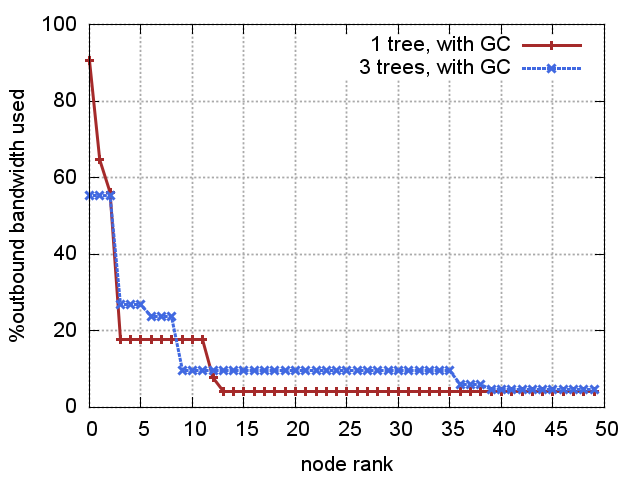
\includegraphics[width=3in]{img/bw-gc.png}
\end{center}
\caption{\label{fig:bw-gc} Outbound bandwidth of each node with data compaction
enabled.  Nodes are sorted in decreasing bandwidth utilization.}
\end{figure}

\begin{figure}[t]
\begin{center}
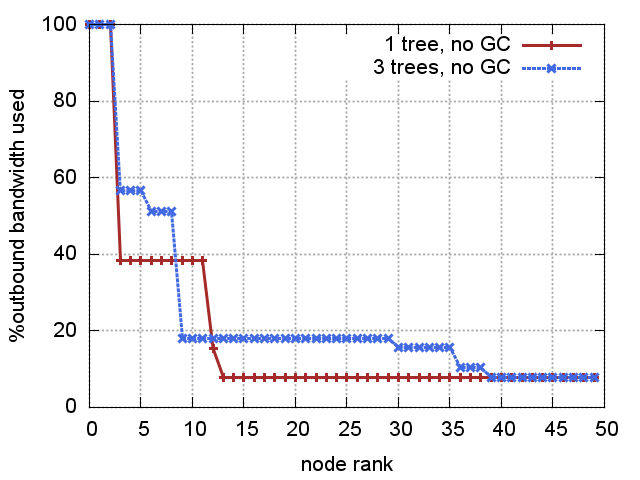
\includegraphics[width=3in]{img/bw-nogc.png}
\end{center}
\caption{\label{fig:bw-nogc} Outbound bandwidth of each node with data
compaction enabled.  Nodes are sorted in decreasing bandwidth utilization.}
\end{figure}

Figure~\ref{fig:bw-nogc} shows the breakdown of outbound bandwidth usage of the
same experiments, but with data compaction disabled.  Without data compaction,
the system cannot handle the large amount of messages generated.  Even with
multiple trees, all the root nodes are being completely saturated.  However,
the use of multiple trees makes extra bandwidth available, and the total amount
of messages sent through the system (represented by the area under each curve,
since no message is discarded) still gets higher.

